% !TEX root = ../main.tex
%

\section{Results}
\label{sec:results}


\subsection{Main findings}
\label{ssec:results:main}

\paragraph{Finding 1: LLM facilitators significantly improve synthetic discussions.} As shown in Fig.~\ref{fig:toxicity_stats}, comments in unmoderated discussions exhibit significantly more intense toxicity. Linear regression on toxicity over time show that the toxicity of trolls decreases by $\minus0.0125$ points on average per discussion turn ($Adj. R^2= 0.413, p=0.003$), although this restraining effect is even more pronounced for neutral and community-oriented users, whose toxicity decreases by $0.0225 (p <.000)$  and $0.0350 (p <.000)$ points per turn respectively. This suggests that the facilitator is effective at steering discussions toward lower toxicity over time, even in the absence of direct punitive mechanisms. While trolls are more resistant to this influence, they still exhibit a measurable decline in toxicity as the discussion progresses.

\begin{figure}
	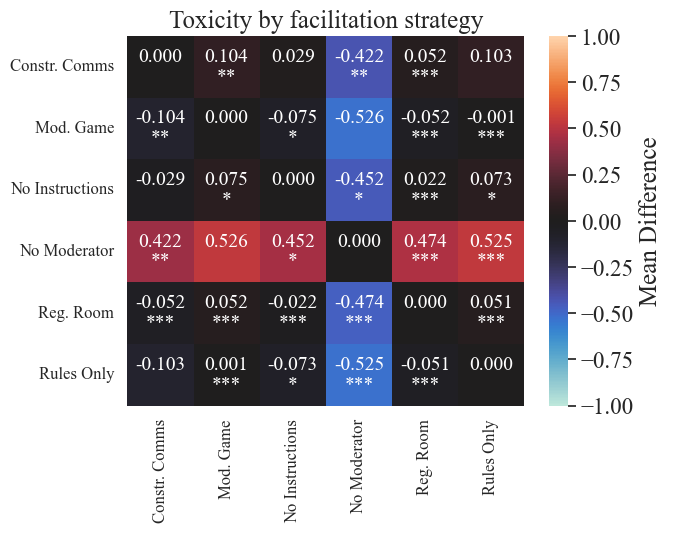
\includegraphics[width=\linewidth]{toxicity_stats.png}
	\centering
	\caption{Difference in average toxicity levels for comments following pairs of facilitation strategies. Red cells ($x>0$) indicate that the strategy on the left performs worse than the one on the bottom, for an average of $x$ points in a scale of 1-5. Conversely for blue ($x<0$) cells. White cells denote minute changes. Asterisks derived from pairwise Student-t tests (\asterisknote). The large size of our dataset allows using parametric tests.}
	\label{fig:toxicity_stats}
\end{figure}

\paragraph{Finding 2: More elaborate facilitation strategies fail to decrease toxicity.}
Strategies such as \emph{\strategyregroom}, \emph{\strategyconstrcomm}, and our proposed \emph{\strategymodgame} significantly reduce comment toxicity compared to \emph{unmoderated} discussions, with their effectiveness increasing over time (Table~\ref{tab:toxicity}). However, these more elaborate facilitation approaches do not consistently outperform the simpler \emph{\strategynoinstr} strategy overall (Fig.~\ref{fig:toxicity_stats}). This suggests that out-of-the-box LLMs may struggle to meaningfully incorporate complex instructions—a limitation noted in prior work \cite{cho-etal-2024-language}. While the real-life strategies show a slight edge over time compared to \emph{\strategynoinstr}, the observed long-term gains are modest and not qualitatively significant in the broader context.

\begin{table}[t]
	\centering
	\begin{tabular}{p{5cm} p{1.5cm}}
		\toprule
		\textbf{Variable} & \textbf{Toxicity} \\
		\midrule
		Intercept & 2.164\textsuperscript{***} \\
		\strategynoinstr & -0.426\textsuperscript{***} \\
		\strategymodgame & -0.435\textsuperscript{***} \\
		\strategyrules & -0.461\textsuperscript{***} \\
		\strategyregroom & -0.277\textsuperscript{***} \\
		\strategyconstrcomm & -0.230\textsuperscript{***} \\
		time & -0.012\textsuperscript{**} \\
		\strategynoinstr$\times$time & -0.003 \\
		\strategymodgame$\times$time & -0.011\textsuperscript{*} \\
		\strategyrules$\times$time & -0.008 \\
		\strategyregroom$\times$time & -0.023\textsuperscript{***} \\
		\strategyconstrcomm$\times$time & -0.023\textsuperscript{***} \\
		\bottomrule
	\end{tabular}
	\small
	\asterisknote
	\normalsize
	\caption{OLS regression coefficients for toxicity on the non-facilitator comments ($Adj. R^2=0.054$). Reference factor is \textit{\strategynomod}. All strategies outperform \textit{\strategynomod} in general. The \textit{\strategyregroom} and \textit{\strategyconstrcomm} real-life strategies additionally show improvements over time compared to \textit{\strategynomod}.}
	\label{tab:toxicity}
\end{table}


\paragraph{Finding 3: LLM facilitators choose to intervene far too frequently, which is tolerated by the other participants.} Fig.~\ref{fig:intervention_count} demonstrates that LLM facilitators intervene at almost any opportunity, even though they are instructed to only do so when necessary. This confirms that LLMs generally can not decide not to speak even when instructed to do so  (\S\ref{ssec:methodology:turn}). To our knowledge, this has not been reported in relevant literature, and \emph{is an example of ``debugging'' problems with LLMs} --- a core motivation of our work.

Additionally, a qualitative look through the dataset reveals that LLM user-agents exhibit atypical tolerance for excessive facilitator interventions. Humans in contrast, typically become irritated and more toxic after repeated, unneeded interventions \citep{schaffner_community_guidelines, make_reddit_great, proactive_moderation, cresci_pesonalized_interventions}. This is likely another artifact caused by alignment procedures, making LLMs too agreeable \citep{park2023game, anthis_2025}.

\begin{figure}[t]
	\centering
	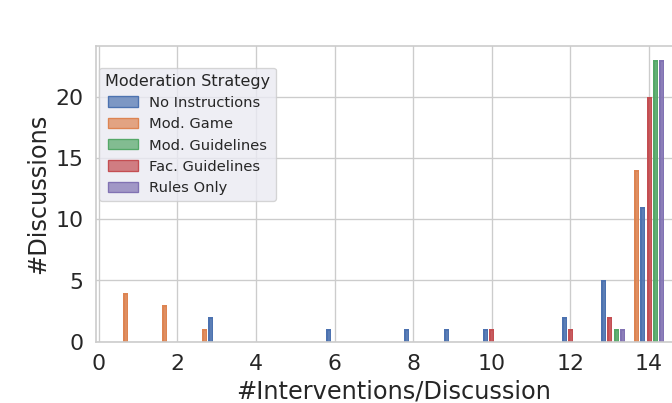
\includegraphics[width=\columnwidth]{intervention_count.png}
	\caption{Histogram of interventions by LLM facilitators per strategy used.}
	\label{fig:intervention_count}
\end{figure}


\subsection{Ablation Study}
\label{ssec:results:ablation}

\begin{figure}[t]
	\centering
	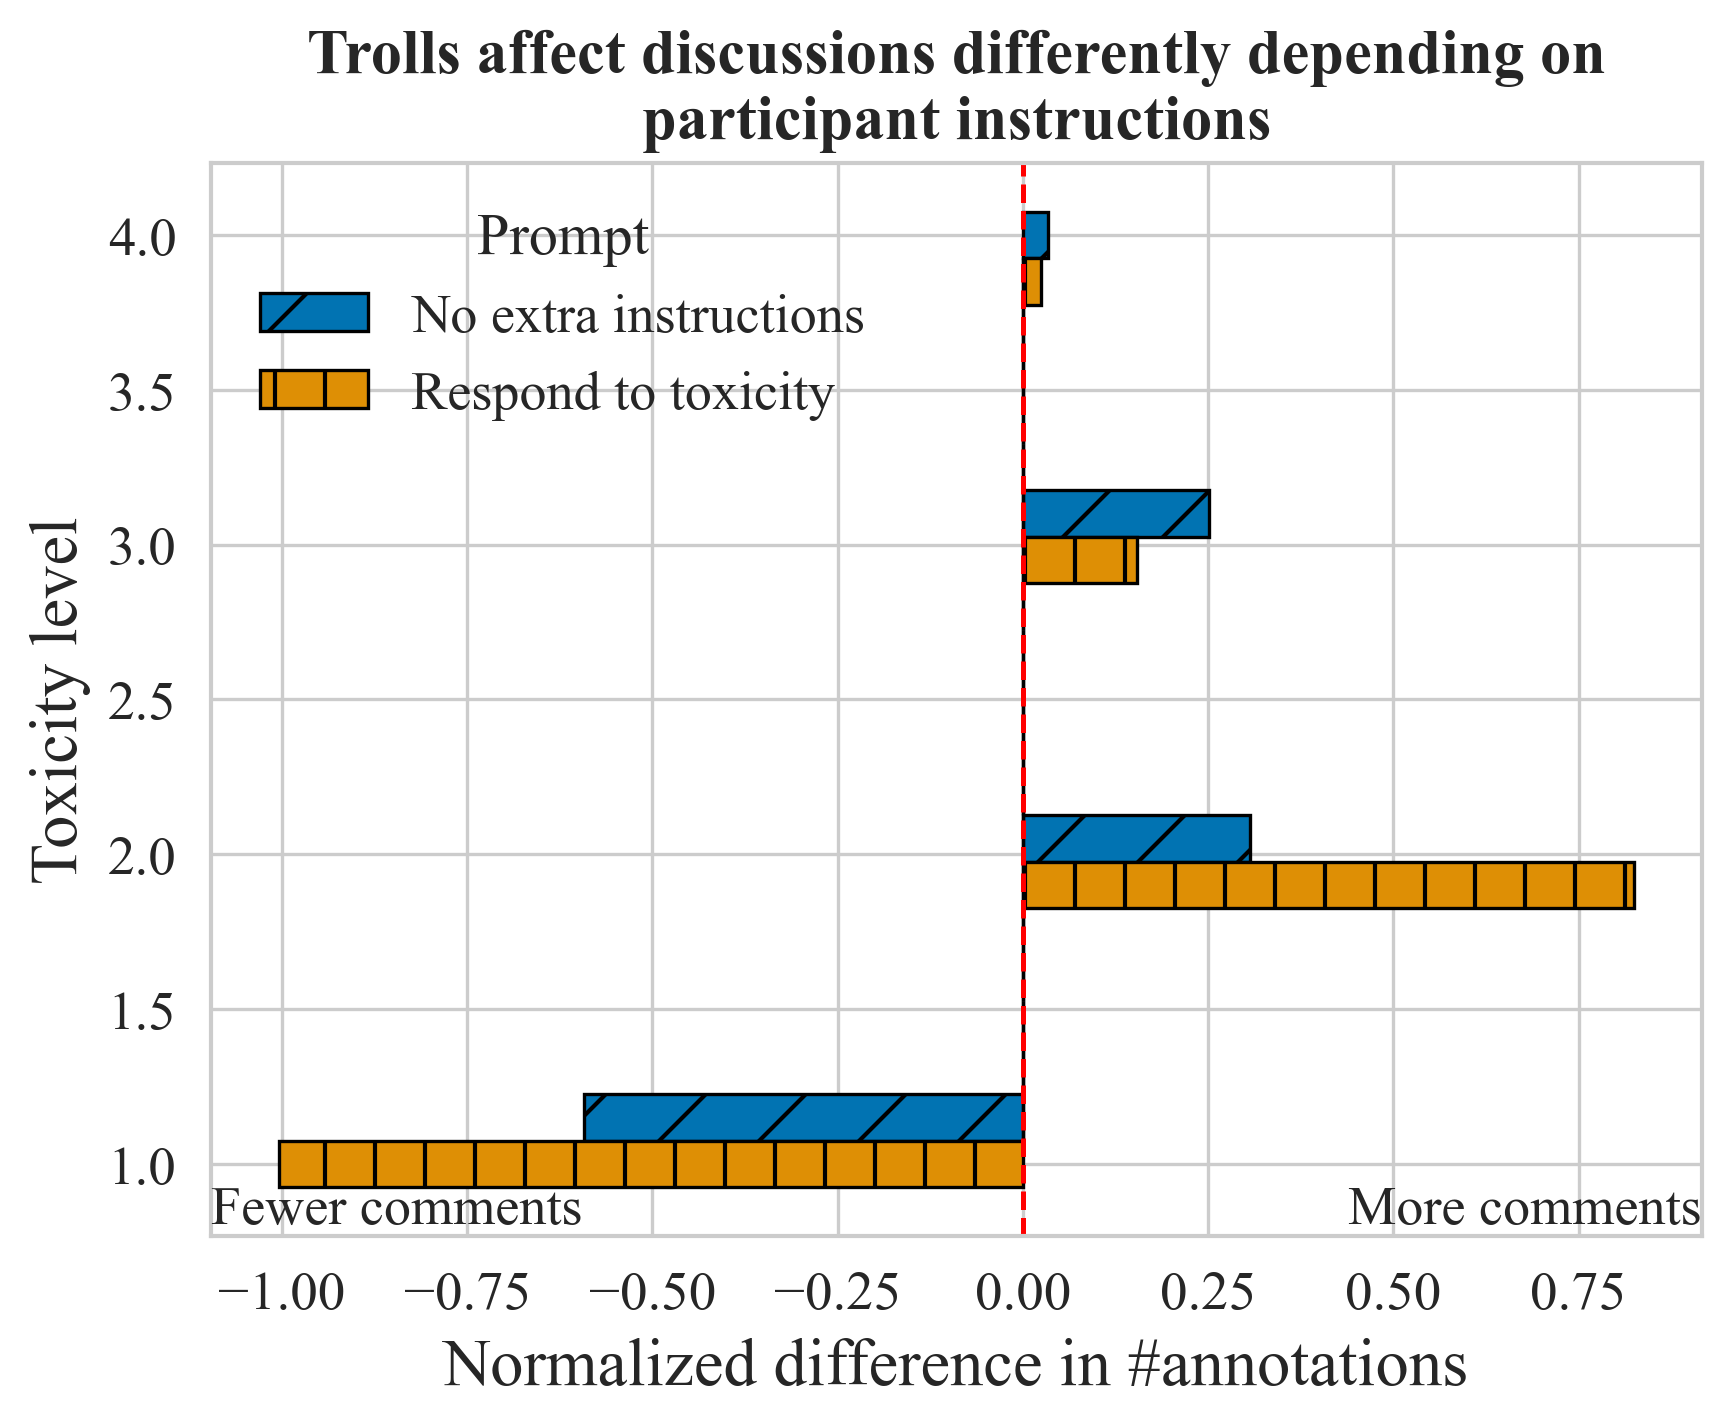
\includegraphics[width=0.8\linewidth]{toxicity_trolls.png}
	\caption{Non-troll toxicity levels in discussions with and without trolls. There is a significant uptick on the number of ``somewhat toxic" ($Toxicity=2$) comments when the participants are primed to respond to toxic comments (lower bars).}
	\label{fig:toxicity_trolls}
\end{figure}

\begin{figure*}[t]
    \begin{subfigure}{0.32\linewidth}
        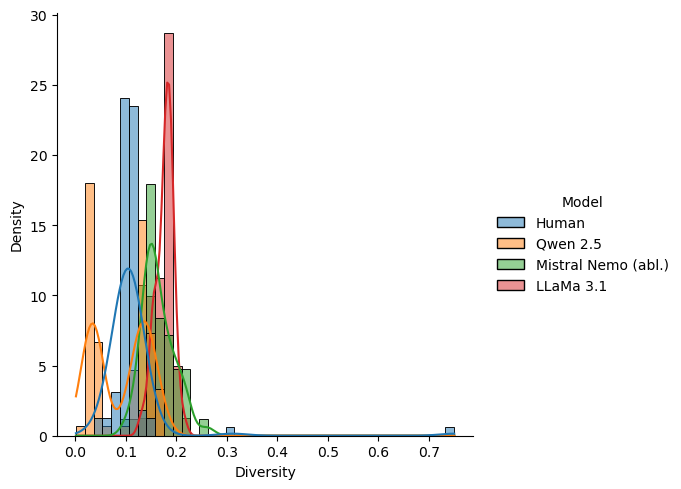
\includegraphics[width=\textwidth]{rougel_model.png}
        \caption{Model}
        \label{fig:rougel_model}
    \end{subfigure}%
    \hfill
    \begin{subfigure}{0.32\linewidth}
        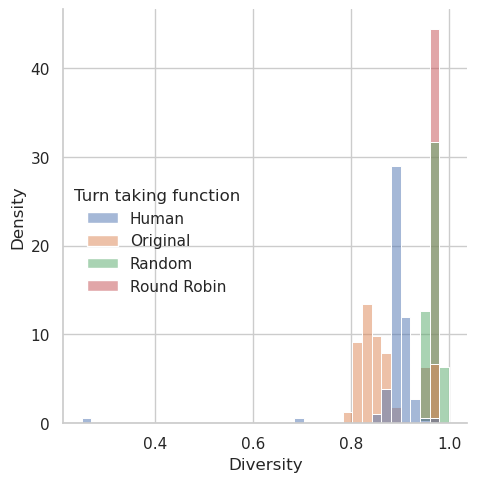
\includegraphics[width=\textwidth]{rougel_turns.png}
        \caption{Turn-taking function}
        \label{fig:rougel_turns}
    \end{subfigure}%
    \hfill
    \begin{subfigure}{0.32\linewidth}
        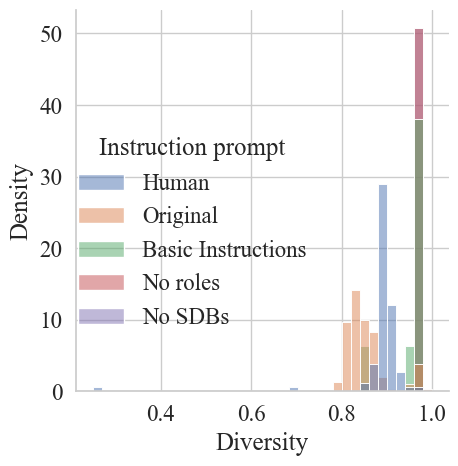
\includegraphics[width=\textwidth]{rougel_prompts.png}
        \caption{Instruction prompt}
        \label{fig:rougel_prompts}
    \end{subfigure}%

    \caption{Diversity (\S\ref{ssec:related:quality}) distribution for each discussion by LLM (\S\ref{ssec:experimental:setup}), turn-taking function $t$ (\S\ref{ssec:methodology:turn}), and prompting function $\phi$ used (\S\ref{ssec:methodology:prompts-instructions}). Comparison with the CeRI Regulation Room dataset (``Human''). Note that the x-axis starts from $0.6$.}
    \label{fig:diversity}
\end{figure*}

We generate eight synthetic discussions per ablation experiment, using a single model (Qwen 2.5). We compare the diversity (cf. \S\ref{ssec:related:quality}, \S\ref{ssec:experimental:evaluation}) of these discussions with ones from the CeRI “Regulation Room” dataset\footnote{Disclaimer: Any opinions, findings, and conclusions or recommendations expressed in this material are those of the author(s) and do not necessarily reflect the views of the CeRI.}. We pick this dataset because it is publicly available and comprised of facilitated online human discussions on ten diverse topics.

\paragraph{Larger models do not lead to more high-quality discussions.} As shown in Fig.~\ref{fig:rougel_model}, Qwen demonstrated the highest diversity among the evaluated models, indicating limited participant interaction (\S\ref{ssec:related:quality}), followed by Mistral Nemo and LLaMa. However, none of the models closely matched the diversity observed in human discussions. 


\paragraph{Our proposed turn-taking function substantially improves the quality of synthetic data.} We compare our turn-taking function (\S\ref{ssec:methodology:turn}) to two baselines: Round Robin (participants speaking one after the other, then repeating) and Random Selection (uniformly sampling another participant each turn). Fig.~\ref{fig:rougel_turns} demonstrates that although all distributions diverge from the blue—human—distribution, our function is the only one not exhibiting extremely high diversity (i.e., very limited participant interaction \S\ref{ssec:experimental:evaluation}).

We conduct three separate experiments in which participants are subjected to one of the following conditions at a time: (1) no assigned SDBs, (2) no assigned roles, or (3) only a very basic instruction prompt given. 

\paragraph{Specialized instruction prompts are essential for eliciting toxic behavior in instruction-tuned LLMs.} Our instruction prompt for the participants (\S\ref{ssec:methodology:prompts-instructions}) incentivizes them to react to toxic behavior. Indeed, inserting “troll” participants to discussions, leads to more intense toxicity among \emph{other} participants \emph{only if we instruct participants to react to toxic posts} (Fig.~\ref{fig:toxicity_trolls}). 

\paragraph{SDBs, roles, and our instruction prompt all increase the quality of synthetic data.} Fig.~\ref{fig:rougel_prompts} illustrates that incorporating SDBs, roles, and specialized instruction prompts, results in diversity scores more closely aligned with human discussions.
